\begin{frame}{simulated misses: BST lookups}
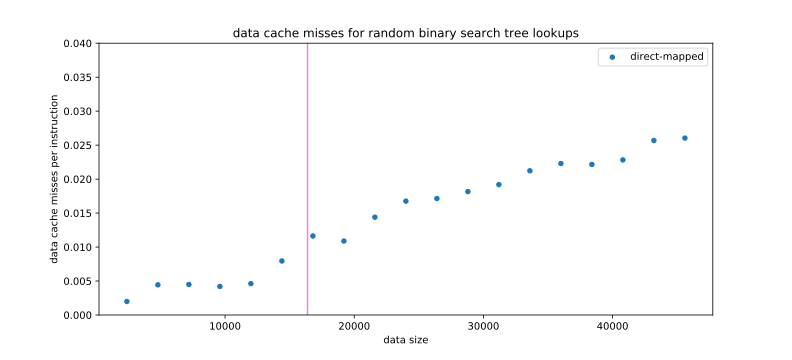
\includegraphics[width=\textwidth]{../caching/bst-one}
(simulated 16KB direct-mapped data cache)
\end{frame}

\begin{frame}{actual misses: BST lookups}
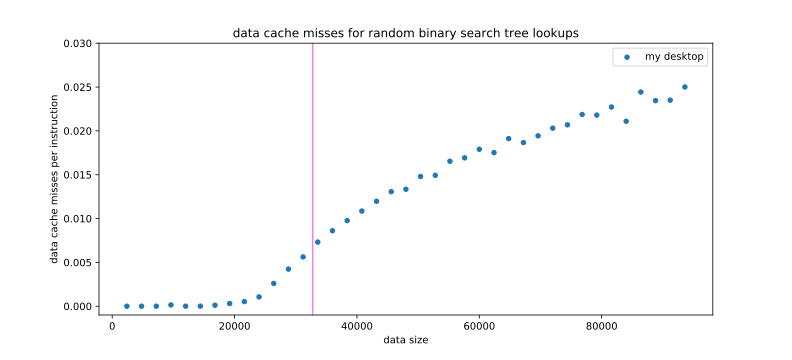
\includegraphics[width=\textwidth]{../caching/bst-act}
(actual 32KB more complex data cache) \\
\small (only one set of measurements + other things on machine)
\end{frame}


\begin{frame}{simulated misses: matrix multiplies}
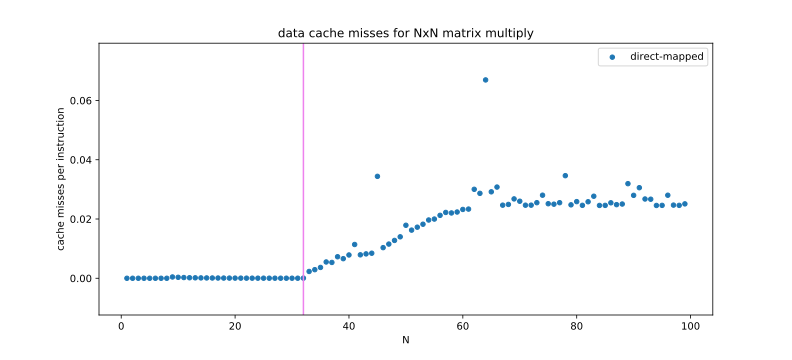
\includegraphics[width=\textwidth]{../caching/mm-one}
(simulated 16KB direct-mapped data cache)
\end{frame}

\begin{frame}{actual misses: matrix multiplies}
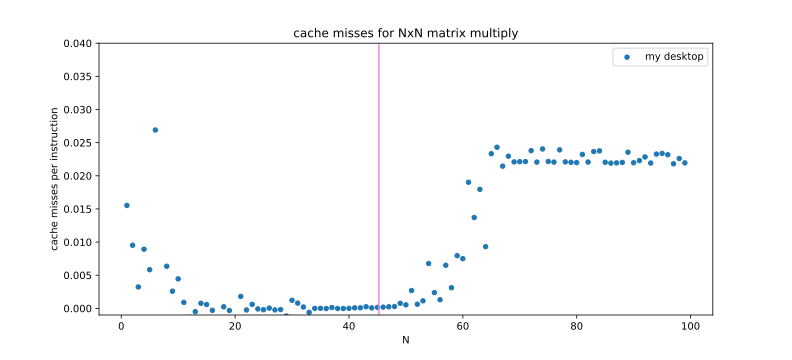
\includegraphics[width=\textwidth]{../caching/mm-act}
(actual 32KB more complex data cache) \\
\small (only one set of measurements + other things on machine)
\end{frame}
